%%%%%%%%%%%%%%%%%%%%%%%%%%%%%%%%%%%%%%%%%%%%%%%%%%%%%%%%%%%%%%%%%%%%%
% PREAMBLE
%%%%%%%%%%%%%%%%%%%%%%%%%%%%%%%%%%%%%%%%%%%%%%%%%%%%%%%%%%%%%%%%%%%%%
%
% The following two commands will generate a PDF that follows all the requirements for submission
% and peer review.  Uncomment these commands to generate this output (and comment out the two lines below.)
%
% DOUBLE SPACE VERSION FOR SUBMISSION TO THE AMS
\documentclass[twocol]{ametsocV5}

%\journal{jpo}
%\linenumbers
\graphicspath{{./figures/}{/Users/jklymak/ForcedChannel5k/figs/}{/Users/jklymak/AbHillParam/python/doc/}}
\DeclareGraphicsExtensions{.pdf}
\usepackage[plain]{fancyref}
\usepackage{xcolor}
\usepackage{amssymb}
\newcommand{\tempS}[1]{}
\newcommand{\twowidth}[0]{4in}
\newcommand{\onewidth}[0]{3.2in}
\newcommand{\mn}[1]{{\sc #1}}
\DeclareGraphicsExtensions{%
    .pdf,.png}
    
\bibpunct{(}{)}{;}{a}{}{,}
% \linenumbers
\newcommand{\myabstract}{}
%
%
%%%%%%%%%%%%%%%%%%%%%%%%%%%%%%%%%%%%%%%%%%%%%%%%%%%%%%%%%%%%%%%%%%%%%
% TITLE
%
% Enter your TITLE here
%%%%%%%%%%%%%%%%%%%%%%%%%%%%%%%%%%%%%%%%%%%%%%%%%%%%%%%%%%%%%%%%%%%%%
\title{Parameterizing non-propagating form drag over rough bathymetry}
%
% Author names, with corresponding author information.
% [Update and move the \thanks{...} block as appropriate.]
%
\authors{Jody M. Klymak \correspondingauthor{Jody Klymak, jklymak@uvic.ca, University of Victoria, Victoria, BC, Canada}}
\affiliation{University of Victoria, Victoria, BC, Canada}

\extraauthor{Dhruv Balwada }
\extraaffil{University of Washington, Seattle, WA, USA}

\extraauthor{Alberto Naveira Garabato}
\extraaffil{National Oceanography Centre, Southampton, United Kingdom}

\extraauthor{Ryan Abernathy}
\extraaffil{Columbia University, New York, New York, USA}



% \email{jklymak@uvic.ca}

\abstract{Slowly evolving stratified mean and eddying flow over rough topography is subject to substantial drag due to the internal motions generated, but often numerical simulations are carried out at resolutions where this ``wave'' drag must be parameterized.  Here we propose a simple parameterization of this drag that has a minimum of fit parameters compared to existing schemes. The parameterization smoothly transitions from a quadratic drag law ($\sim hu_0^2$) for low-$Nh/u_0$ (linear wave dynamics) regimes to a linear drag law ($\sim h^2 u_0 N$) for high-$Nh/u_0$ flows (blocking and hydraulic dynamics) , where $N$ is the stratification, $h$ is the amplitude of the topography, and $u_0$ is the near-bottom velocity; the parameterization does not have a dependence on Coriolis frequency.  Simulations carried out in a channel with synthetic bathymetry and steady body forcing indicate that this parameterization predicts drag across a broad range of forcing parameters.  The parameterization is also tested in more realistic simulations of wind-driven channels that generate mesoscale eddy fields, a setup where the mean downstream transport is very sensitive to the bottom drag parameterization and its effect on the eddies.  In these simulations, the parameterization is found to replicate the effect of rough bathymetry both on the eddies and the mean flow, but the value of $h$ must be doubled over the value used in the steady simulations for the best agreement.}  

\begin{document}

\maketitle

%%%%%%%%%%%%%%%%%%%%%%%%%%%%%%%%%%%%%%%%%%%%%%%%%%%%%%%%%%%%%%%%%%%%%
% MAIN BODY OF PAPER
%%%%%%%%%%%%%%%%%%%%%%%%%%%%%%%%%%%%%%%%%%%%%%%%%%%%%%%%%%%%%%%%%%%%%
\section{Introduction}

Stratified flows passing over bathymetry experience drags that are often many orders of magnitude larger than that due to skin friction alone due to the creation of internal motions that either radiate away as internal waves \citep{bell75a} or are trapped as ``non-propagating'' motions near the topography \citep[i.e.][]{bacmeisterpierrhumbert88}.  Including these motions in large-scale models is important to the momentum balance and mixing in both the ocean and the atmosphere, and must be parameterized if simulations do not include enough resolution to capture the small-scale topography.  

Here we consider low-frequency flows, where the variation in the flow is taken to be substantially sub-inertial and has a given near-bottom speed $u_0$.    The flow is taken to be over idealized topography that is stochastically specified by empirical models in the form given by \citet{goffarbic10}, rather than over any sort of realistic topography.    In this situation, there are two simple parameters controlling the flow regimes found.  First, for high-wavenumber $k$ parts of the topography where $u_0k > f$ radiating internal lee waves are possible because the intrinsic frequency is greater than $f$.  If the second parameter $Nh/u_o \lesssim \pi$, where $N$ is the near-topography stratification and $h$ is the amplitude of the topography, then linear theory applies and the drag on the mean flow can be analytically calculated \citep{bell75a}.  The high-wavenumber part of the topography typically has a small amplitude (so-called ``abyssal hills'') so the flows are well-approximated by linear theory \citep{nikurashinferrari10a,nikurashinferrari14}.  The radiated waves interact via wave-wave interactions to cause a halo of turbulence in a region near the sea-floor that is a few hundred meters deep, and amenable to prediction by weakly non-linear theory \citep{polzin09}.  Substantial recent work indicates that parameterizing the ``abyssal hills'' can alter the large-scale circulation and stratification \citep[i.e.]{meletetal13, de_Lavergne_2017}.  

For larger-scale topography ($u_0k<f$) the internal motions cannot radiate as internal waves and, in the linear limit, only remove energy when the flow changes as an evanescent response is set up, and hence this drag is termed ``non-propagating''.  However, the topographic spectra are typically red, and hence the amplitudes $h$ appropriate at these scales tends to be substantially larger than for high-$k$ topography, and $Nh/u_0$ can become quite large.  The flow at this scale is thus inherently non-linear and there is substantial local blocking upstream of topographic features, and breaking downstream. For the oceanic situation \citet{klymak18} demonstrates that for a typical bathymetric spectrum  \citep[i.e.\ the ones used by][]{nikurashinferrari14} the large-scale bathymetry was responsible for 2/3 of the total dissipation in the flow, and hence is crucial to include in parameterizations.  

The importance of parameterizing drag and turbulence due to non-propagating motions over and around large-amplitude topography ($Nh/u_0 >> 1$) has been long realized by the atmospheric science community, and the enhanced mountain drag is imperative to properly simulate the atmosphere \citep[i.e.][]{bacmeisterpierrhumbert88,LottMiller97}.  A number of schemes have been devised based on the fact that substantial portions of the flow can be blocked around an isolated obstacle, and hence the drag become quadratic with the flow speed, and proportional to the cross-sectional area of the obstacle exposed to the mean flow \citep[i.e.][]{ScinoccaMcFarlane00, Garner05}.  These parameterized drags have been shown to be important in numerical simulations of the ocean \citep{trossmanetal13,trossmanetal2016}, and to have promise when compared to observations \citep{TrossmanEtAl15}.  These parameterizations are quadratic in flow speed and linear in obstacle height corrected by the blocking depth $h_b = u_0/N$
\begin{equation}
    D_{np} \sim (h-h_b)\ u_0 \left|u_0\right|.
\end{equation}
Conversely, \citep{klymaketal10a} found that drag for $Nh/u_0 >> 1$ is linear in $u_0$ and quadratic in height for a two-dimensional obstacle:  
\begin{equation}
    \frac{D_{np}}{\rho_0} \approx \frac{u_0^2\, h}{L}\, \frac{\pi}{2}\left[\frac{N h}{u_0}+ \pi\right] = C_l u_0 + C_q u_0^2,
    \label{eq:FormDragParam}
\end{equation}
where $L$ is an along-flow lateral scale (discussed below), and we have defined a linear drag co-efficient as $C_l = \frac{N h^2\pi}{2L}$ and a quadratic drag co-efficient as $C_q = \frac{h\pi^2}{2L}$.  Note that the quadratic  term has the same scaling as the non-linear drag typically used in the atmosphere for low $Nh/u_0$.  

The goal of this paper is to test the appropriateness of the parameterization in \fref{eq:FormDragParam}, and argue that it provides an accurate yet simple way to transition between high- and low-$Nh/u_0$ flow regimes with a minimum of fit parameters.  It was shown in \citet{klymak18} that the non-propagating drag is indeed linear in the flow speed $u_0$, and not quadratic.  Here we test the rest of the parameterization both via idealized simulations that also vary $N$, $h$, and the Coriolis parameter $f$, and by testing the parameterization with more realistic, but still idealized, wind- and thermally forced channel flows.  After specifying the numerics used in the simulations (\fref{sec:Model}), we argue that \fref{eq:FormDragParam} is indeed appropriate across a large range of parameters (\fref{sec:ResultsSingleFlow}).  The paper subsequently considers a large number of simulations that are idealizations of the flow in the Southern Ocean  (\fref{sec:ResultsWindForcing}).  The wind-driven channel was chosen for testing the parameterization because it is a closed system that still demonstrates substantial complexity that may be met by an eddy-resolving large-scale simulation, and there is substantial literature that uses it already \citep[i.e.][]{abernatheycessi14,Marshall_2017}.   
 




%\citet{klymaketal10a}
\section{Model configurations}
\label{sec:Model}

Two types of simulation are used in this paper.  The first is a doubly-periodic domain forced with a cross-channel body force that, absent other forces, is geostrophically balanced by an along-channel flow.  Stratification, topographic roughness, and Coriolis frequency are varied to test the parameterization of the near-bottom drag.  The second configuration is a long re-entrant channel that has a large Gaussian ridge in the middle and varying roughness.  This model is forced with a wind stress and thermal relaxation at the surface, and the bottom drag is either resolved or parameterized.  

The \verb+MITgcm+ was used for all simulations \citep{marshalletal97}, in a manner analogous to previous work at similar scales \citep{buijsmanetal14,klymaketal16b, klymak18}.  Background explicit vertical and horizontal viscosity and diffusivity are kept low ($K_{\rho} = \nu = 10^{-5}\ \mathrm{m^2\ s^{-1}}$) except in the presence of resolved density overturns where the vertical viscosity and diffusions are increased in a manner consistent with the expected Thorpe scale \citep{klymaklegg10}.  There is also numerical diffusivity and dissipation due to the second-order flux-limiting temperature advection scheme (\verb+tempAdvScheme=77+; see the MITgcm manual).  Using a weak explicit diffusivity allows the internal wave field to evolve freely to the extent that the chosen resolution allows, rather than adding artificial damping \citep{ShakespeareHogg17}.  For the work carried out here, the terms in the energy budget are all calculated and the residual is identified as the dissipation.  However, the spatial distribution of explicit dissipation (calculated from the explicit viscosities and local shears) is similar to the spatial distribution of the residual of the energy budget.  The model is run in hydrostatic mode for all simulations.  

\subsection{Doubly periodic, idealized forcing}

These simulations are identical to this used in \citet{klymak18}, and inspired by \citet{nikurashinferrari14}.  We assume a doubly periodic domain with constant stratification and a mean flow in the x-direction forced over rough topography.  The strength of the flow maintained by a body force meant to simulate an externally imposed surface pressure gradient.  The doubly periodic lateral domain of 409.6 km in x, and 118.4 km in the y direction is chosen to capture enough variance in the large-scale topography. All simulations had vertical resolution of 10 m over 4000 m depth.  1-km scale runs were spun up for 200 h.

The topography is the low-passed version of that used in \cite{klymak18} with parameters given by: 
\begin{equation}
    P_{2D}(k,l) = \frac{2\pi h^2 \left(\mu-2 \right)}{k_0l_0}\left( 1 + \frac{k^2}{k_0^2} + \frac{l^2}{l_0^2}\right)^{-\mu/2}
    \label{eq:topo2d}
\end{equation}
where $h$ is the root-mean-square of the topographic height, $\mu=3.5$ is a parameter setting the high-wavenumber slope of $-1.75$, and $k_0=l_0 = 1.8\times10^{-4}\ \mathrm{rad\,m^{-1}}$ are parameters that set the wavelength at which the spectrum of the topography starts to flatten out towards white low-wavenumber spectrum.  A range of values for $h$ were tested, $N$, the background stratification, $k_0$ the roll-off wavenumber, and $f$ the Coriolis parameter.  

% TODO: make a plot of body-forced domain

\subsection{Wind-forced channel simulations}

The second set of simulations are run in a zonal channel forced by a sinusoidal wind stress and temperature relaxation at the surface.  The wind-forced domain has the same numerics as the simulations above.  The channel is 1024 km wide and 1600 km long (\fref{fig:ModelSetup}).  The bathymetry is 3000 m deep, with sloping walls along the north and south wall faces, and a Gaussian ridge in the middle of the domain with a lateral scale of 100 km and a height of 1000 m, so that the shallowest point on the Gaussian is at 2000 m depth.  Simulations are made with smooth seafloor bathymetries, and bathymetries with a roughness added to them that follow the same statistics as in the previous section (\fref{fig:Bathys.pdf}).  These runs are started with a uniform temperature of 4 degrees C, and the temperature is forced at the surface with a relaxation time scale of 48 hours to be $4^o\mathrm{C}$ at the southern end, and linearly increasing to $12^o\mathrm{C}$ at the northern.  A sinusoidally varying wind forcing is also applied down-channel, with a peak in the middle of $0.2\ \mathrm{Pa\ m^{-2}}$, and nulls at the north and south walls.  This forcing and setup is meant to emulate many wind-driven channel studies \citep[i.e.][]{abernatheycessi14, Marshall_2017}.  


\begin{figure}[htbp]
  \begin{center}
    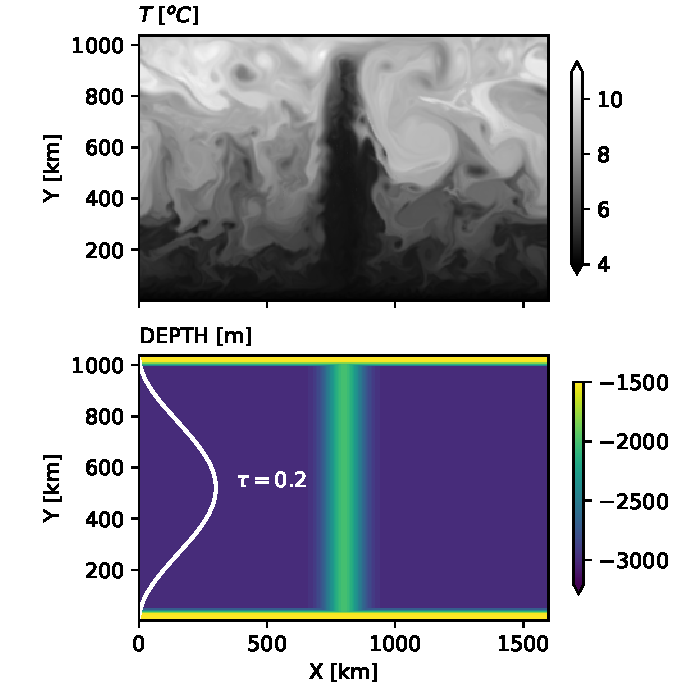
\includegraphics[width=\onewidth]{ModelSetup}
    \caption{Wind forced channel configuration.  
      \tempS{\footnotesize /Users/jklymak/leewaves17/doc//PlotEnergyCoarse.ipynb ;     
        /Users/jklymak/leewaves17/doc/SnapsRegrid2U.pdf}
      \label{fig:ModelSetup} }
  \end{center}
\end{figure}



\begin{figure}[htbp]
  \begin{center}
    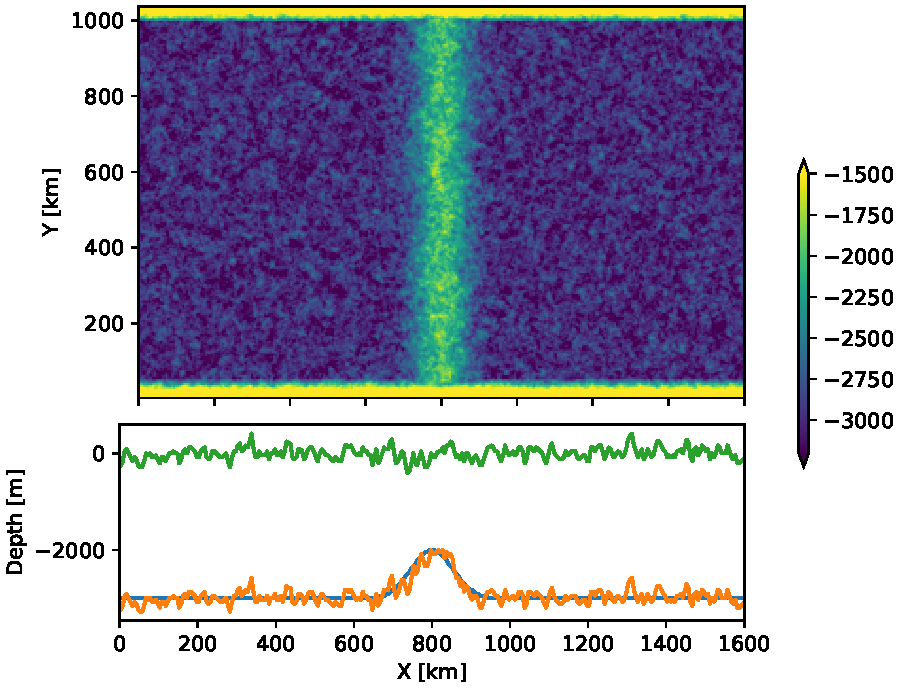
\includegraphics[width=\onewidth]{Bathys.pdf}
    \caption{Wind-forced channel bathymetry, with stochastic roughness added. 
      \tempS{\footnotesize ../figs///Notes5k ;
        ../figs//Bathys.pdf.pdf}
      \label{fig:Bathys.pdf} }
  \end{center}
\end{figure}

These simulations were run in stages; a 20 km horizontal resolution and 80-m vertical simulation was made for 100 years of simulation time with the smooth bathymetry.  A second run was made with the lateral resolution increased to 5-km, and the vertical resolution increased to 40 m for 10 years. 5-km was the limit of what we could feasible simulate with modest computing resources, and the indication from \citet{klymak18} is that this resolution will provide a drag in flows with rough bathymetry that is probably exaggerated by a factor of 1.4 compared to simulations with  100-m x 10-m resolution.     
As noted below, the simulations are close to being in mechanical equilibrium, but they are not anywhere near thermal equilibrium, which would require a few centuries of simulation \citep[i.e.][run similar simulations for 620 years]{Munday_2015}.   

\section{Parameterizing drag due to large-scale lateral topography}
\label{sec:ResultsSingleFlow}


\begin{figure*}
  \begin{center}
    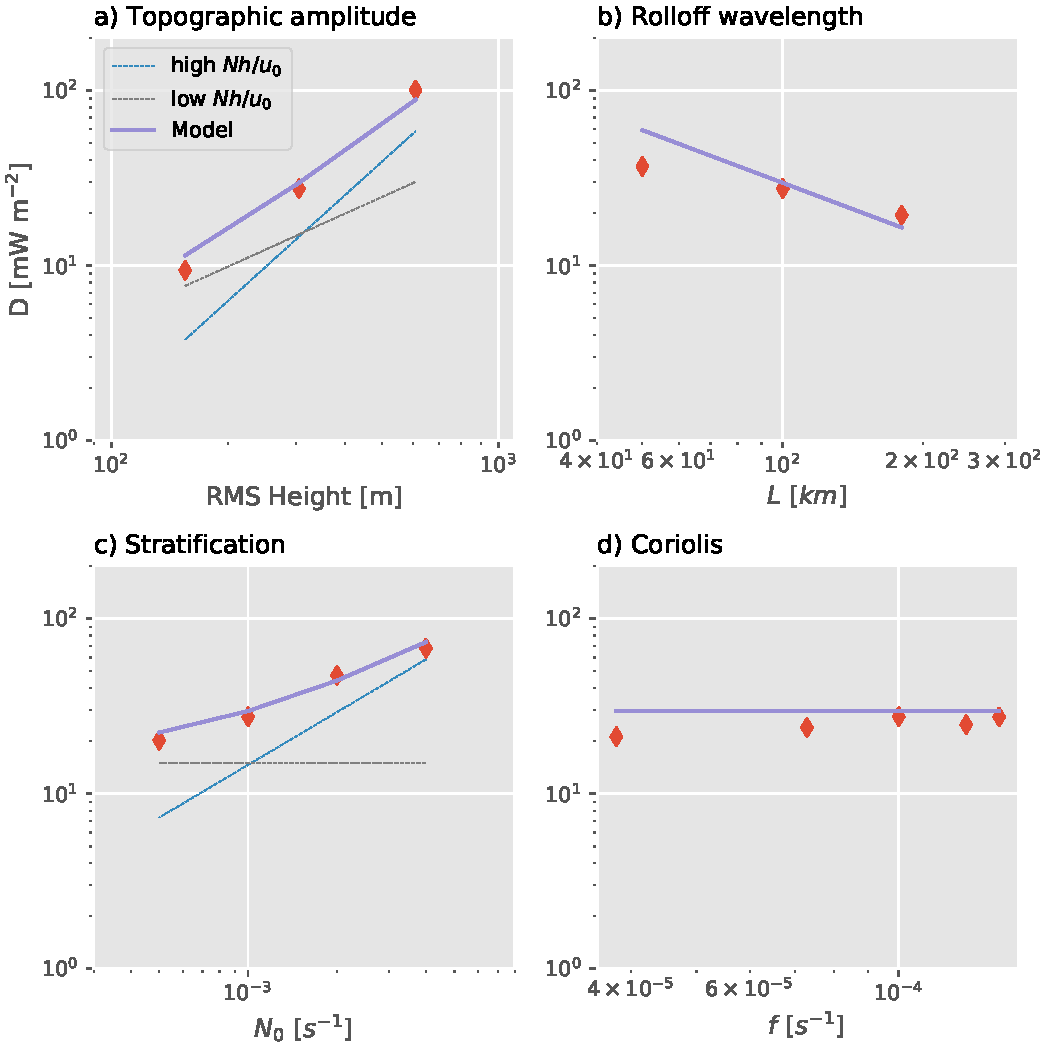
\includegraphics[width=\twowidth]{PowerlawDep}
    \caption{Dependence of simulations on varying a) stochastic topographic amplitude; b) the roll-off wavelength at which the topographic amplitude starts to fall off; c) the stratification, and d) the Coriolis parameter.  In each panel, the expectation from the model given by \fref{eq:FormDragParam} is indicated, with both the high- and low-$Nh/U$ asymptotes shown as thin dashed lines.
      \tempS{\footnotesize /Users/jklymak/leewaves17/doc//PlotEnergyCoarse.ipynb ;     
        /Users/jklymak/leewaves17/doc/SnapsRegrid2U.pdf}
      \label{fig:PowerlawDep} }
  \end{center}
\end{figure*}

The first series of simulations were run with a body force over doubly-periodic stochastic topography similar to \citet{klymak18} where here we only consider topography low-passed in space so that variance at scales smaller than 6-km is attenuated.  At smaller scales, linear lee-wave parameterizations tend to do well, so we are only interested in parameterizing the large scales here.  For comparison with the parameterization (\fref{eq:FormDragParam}), we choose a representative horizontal spacing between obstacles as $L = \left(100 \ \mathrm{km}\right) 1.8 \times 10^{-4}\ \mathrm{rad\ m^{-1}} / k_0$, where $k_0$ is the roll-off wavenumber of the topographic spectrum \citep{klymak18}.  Simulations were run with a base configuration of $f=10^{-4}\ \mathrm{rad\, s^{-1}}$, $u_0=0.1\ \mathrm{m\,s^{-1}}$, $N=10^{-3}\ \mathrm{rad\, s^{-1}}$, a maximum depth of $H=4000\ \mathrm{m}$ and a topographic roughness on top of this as described by \fref{eq:topo2d} with a basic amplitude of $h = 305\ \mathrm{m}$, $k_0 = l_0 = 1.8\times10^{-4}\ \mathrm{rad\ m^{-1}}$. Energy budgets were performed on the runs, as described in \citep{klymak18}, and an average vertically integrated dissipation rate across the domain was computed as the integral of $v F_b$, where $F_b$ is the y-direction body force used to force the model and $v$ the north-south velocity.


Simulations were then carried out as deviations from the base values.  First $h$ was varied, with $h = 155,\ 305$ and $610\ \mathrm{m}$ (\fref{fig:PowerlawDep}a) we find that higher obstacles lead to more dissipation.  The scaling is definitely steeper with $h$ than linear, and there appears to be some curvature to the response with $h$, as predicted.  We are limited from going to smaller scale topography by the vertical resolution of the model setup.  


As the length scale $L$ is changed by varying  $k_0$ (\fref{fig:PowerlawDep}b) we see that there is less dissipation as the length scale gets larger, as expected, though the dissipation appears to plateau as the obstacles get closer together.  This is likely because the peaks become close to a Rossby radius apart and the topographic elements become less distinct.  

As stratification is increased, $N = 0.5,\ 2,\ 4\times 10^{-3}\ \mathrm{rad\, s^{-1}}$ (\fref{fig:PowerlawDep}c), we see that dissipation goes up, as predicted.  This is the starkest difference with the non-propagating drag parameterizations used in previous literature, which do not account for stratification.  These simulations show that for  larger values of $Nh/u_0$, the stratification definitely plays a leading order role.  

There appears to be, at most, a weak dependence on the Coriolis force: $f$ (\fref{fig:PowerlawDep}d), again as predicted by \fref{eq:FormDragParam}, where there is no dependence on the Coriolis parameter.  The agreement is not perfect; there is a 30\% drop in dissipation as the Coriolis parameter drops to the value that corresponds to 15 N.  However here we have again not changed the topography, so as $f$ drops more internal waves are able to radiate rather than being blocked, a complication we have not tried to account for.  

Finally, \citet{klymak18} showed a clear dependence to $u_o$  that follows that predicted by \fref{eq:FormDragParam}, so we do not reproduce that here.

Overall, the parameterization appears to do a good job over a wide range of ocean-relevant conditions.  It has the advantage over other schemes in that there is only one ad-hoc parameter, and that it allows a seamless merging of the parameterization for high- and low-$Nh/u_0$ flows without arbitrary cut-off parameters.  Conversely, the parameterization does not include the high-wavenumber component of the topography, and hence misses the internal-wave dissipation, but again, there have been robust attempts at addressing  that portion of the drag problem already \citep{nikurashinferrari14}. 

\section{Wind-forced Channel Parameterization}
\label{sec:ResultsWindForcing}

The doubly periodic simulations forced via a body force are not very applicable to the abyssal ocean, where mean flows tend to be dominated by eddying flows on sub-inertial time scales.  So here we test in a wind- and thermally driven simulation that has all the physics forced just at the surface, allowing the near-bottom drag to evolve on its own, and allowing buoyancy to be replenished by the overturning circulation in the channel.  The simulation chosen was a wind-forced re-entrant channel with relaxation of the surface temperature to a north-south gradient, and a large-scale Gaussian ridge in the middle of the channel.  This style of simulation catalyzes eddies in the flow \citep{abernatheycessi14}, and has been shown to be very sensitive to the parameterization of the bottom drag \citep{Marshall_2017}.  

Simulations were made that had roughness down to the 6-km scale, and these were compared to simulations that had the drag due to that roughness parameterized using \fref{eq:FormDragParam}.  As noted above, a smooth version of the model was run for 100 years at 20-km resolution, and then at 5km for 10y.   The expectation, following \citet{Marshall_2017}, is that the rougher bathymetry, and simulations where the roughness is parameterized, will have faster spin down of the eddies, more baroclinicity, and hence stronger downstream transport.  

The smooth bathymetry was run with either a weak quadratic bottom drag ($C_q = 10^{-3}$), or with a bottom drag based on the parameterization above (\fref{eq:FormDragParam}), meant to simulate the drag effect of the rough bathymetry. This was implemented as a quadratic plus linear drag in the model using an approximate stratification at the bottom for $N\approx 5\times10^{-4}\ \mathrm{rad / s}$, the amplitude of the topography at $h_0 = 305\ \mathrm{m}$, and a lateral scale of 100 km, yielding for the base run a linear co-efficient of $C_l = 7.3\times 10^{-4}$ and a quadratic co-efficient of $C_q = 1.5\times 10^{-2}$.    A better parameterization would be to make the coefficients depend on the observed near-bottom stratification, rather than choosing a value for $N$, however, that complexity was not addressed in these simulations.  
\begin{figure*}[htbp]
  \begin{center}
    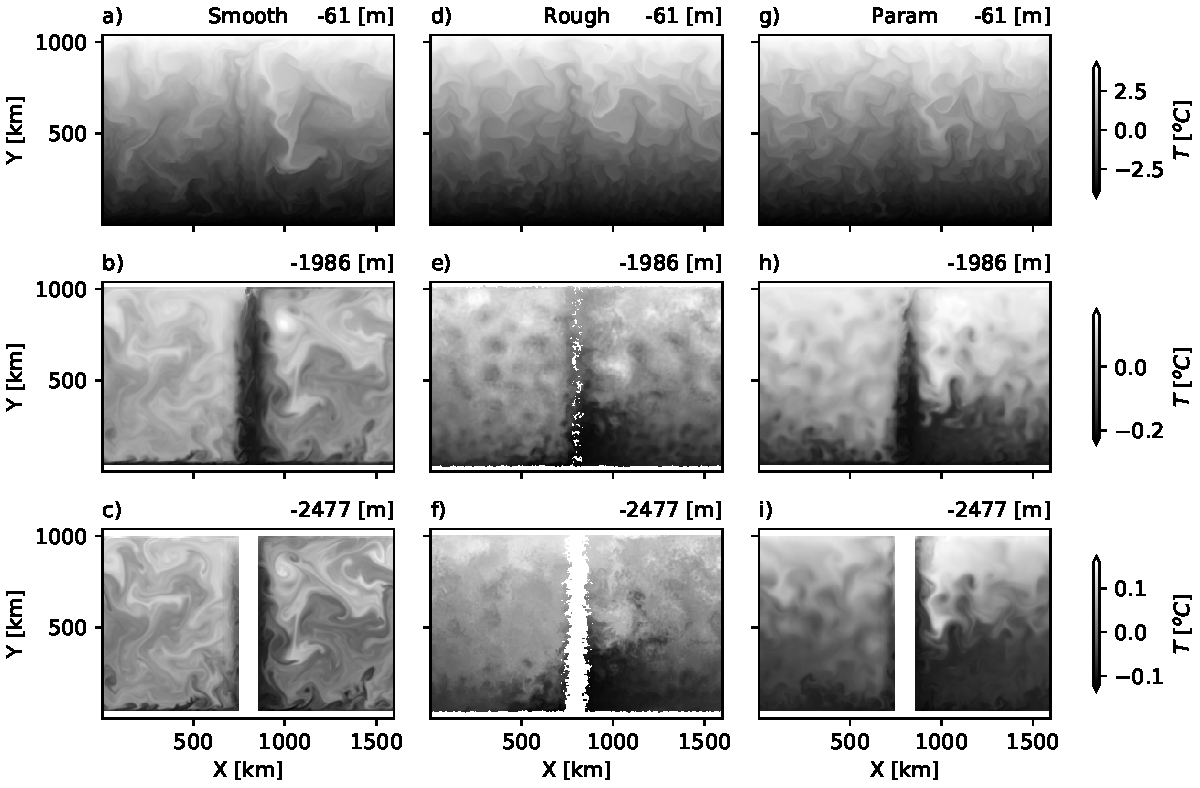
\includegraphics[width=6in]{ExampleTemps}
    \caption{ Example lateral temperature slices (as anomalies from the mean at that depth) through the simulations at depths of -61 m, -1986 m, and -2477 m, with {\sc Smooth} bathymetry in the first column, a synthetic {\sc rough} bathymetry in the second column, and an enhanced parameterized drag in the third column.  
      \tempS{\footnotesize ../figs///Notes5k ;
        ../figs//ExampleTemps.pdf}
      \label{fig:ExampleTemps} }
  \end{center}
\end{figure*}

A second important change was made to these simulations.  Typically the linear and quadratic drags are applied at the bottom-most cell of the simulation.  However this leads to excessive near-bottom shear, and does not slow the water down over the range of depths that it does in the simulations with rough bathymetry.  In order to simulate this effect, the bottom drag is evenly distributed over the bottom 7 grid cells, or over a vertical scale of about 280 m, similar to the vertical blocking scale of the topography $\pi u_0/N$ \citep{klymaketal10a}.  This is similar to what is done by \citet{trossmanetal2016} who applied their non-propagating drag over the bottom 500 m.  

\subsection{Flow response}

Example lateral slices of temperature through the simulations show similar features between the {\sc smooth} and {\sc rough} simulations (\fref{fig:ExampleTemps}), but small-scales are suppressed in the {\sc rough} simulation leading to a more ordered eddy field near the surface as the cascade to small scales is hampered. The {\sc param} simulation has similarly suppressed eddy filamentation.  Note that all three simulations have different mean temperatures at these depths, a symptom of the fact that none of the runs are in thermal equilibrium.  

Spectra of vertical velocity (\fref{fig:Spectra2D}) clearly show the suppression of eddies at subinertial frequency in the {\sc rough} and {\sc param} simulations.  Note the relatively weak internal wave field in all three simulations, which is unsurprising because any trapped internal waves would be sub-inertial in the Eulerian frame of reference, and the usual sources of propagating internal wave energy are missing.  

\begin{figure*}[htbp]
  \begin{center}
    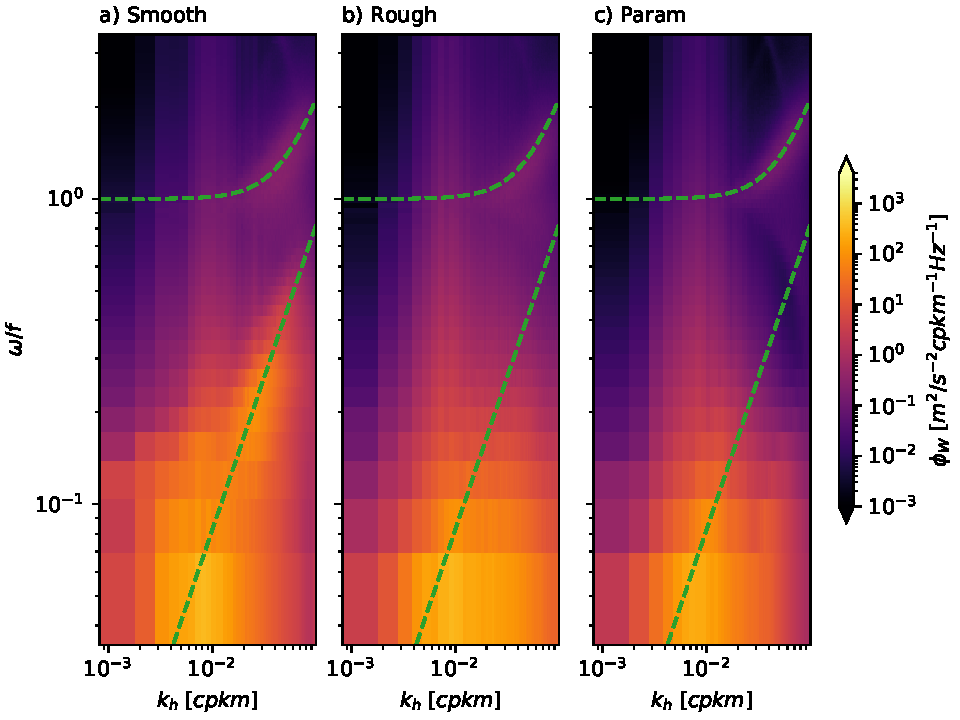
\includegraphics[width=\twowidth]{Spectra2D}
    \caption{Two-dimensional spectra of vertical kinetic energy at -1986 m for the three main simulations.  The dashed green lines are a mode-1 internal wave dispersion relation (at super-inertial frequencies) and eddy motion assuming eddy propagation speeds of 8 km/d.  
      \tempS{\footnotesize ../figs///Notes5k ;
        ../figs//Spectra.pdf}
      \label{fig:Spectra2D} }
  \end{center}
\end{figure*}

The effect on the large-scale flow is as predicted by other studies  \citep[i.e.][]{Marshall_2017}.  Suppressing the mesoscale eddy field increases the baroclinicity of the flow significantly, as well as deepening the thermocline (\fref{fig:UTempCont}).  The reason for this is that eddies are necessary to transmit surface stress down through the water column to eventually be removed at the bottom.  If the eddies are spun down more quickly, the flow must develop more baroclinicity, and hence more baroclinic instability,  until enough eddy stress exists to allow the flow to come into steady state.  A byproduct is that there will be a stronger near-surface flow, and an increase the transport in the channel (see below).   

\begin{figure}[htbp]
  \begin{center}
    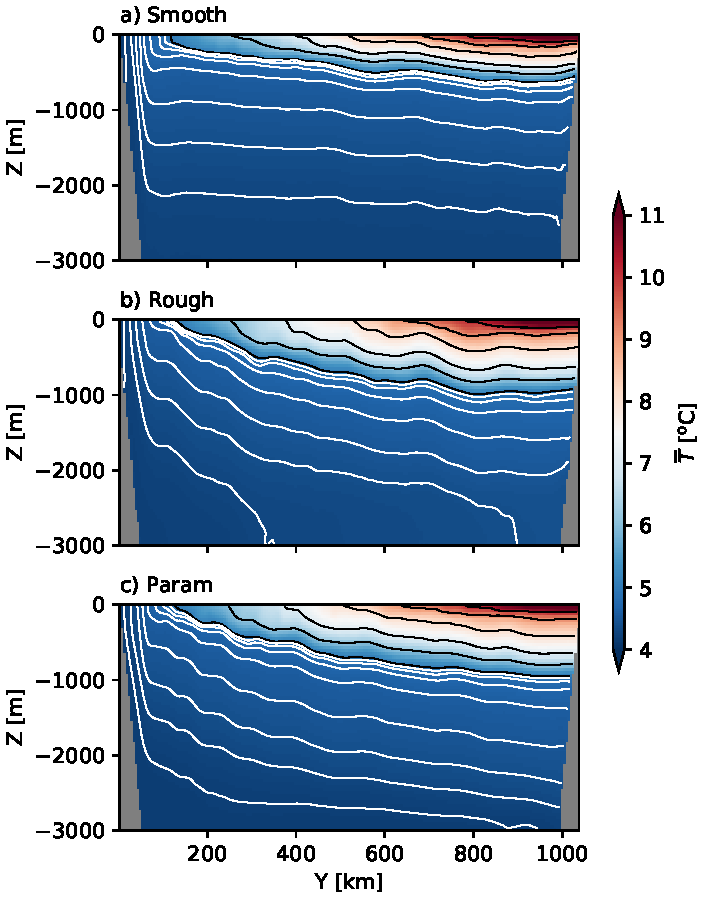
\includegraphics[width=\onewidth]{UTempCont}
    \caption{Zonal temperature sections, averaged from x=0 to 500 km. Black contours are every degree C, white contours every 1/10 degree C from 5 to 4 degrees for three simulations a) {\sc Smooth} bathymetry, b) {\sc Rough} bathymetry and c) smooth bathymetry with the "double-h" parameterization.  
      \tempS{\footnotesize ../figs///Notes5k.ipynb ;
        ../figs//UTempCont.pdf}
      \label{fig:UTempCont} }
  \end{center}
\end{figure}

An interesting effect of the rough bathymetry (and its parameterization) is to greatly alter the standing meander that forms directly downstream of the basin-scale Gaussian ridge, most clearly seen by looking at the bottom pressure signal (\fref{fig:BottomPressure}).  There is low pressure over the ridge in all three simulations, but downstream, the large anti-cyclone is not as strong in the {\sc rough} and {\sc param} simulations.  The effect of this on the large-scale drag is beyond our scope here, but is a curious result of adding more friction to the bottom drag \citep[i.e.]{thompsonnaveiragarabato14}.

\begin{figure}[htbp]
  \begin{center}
    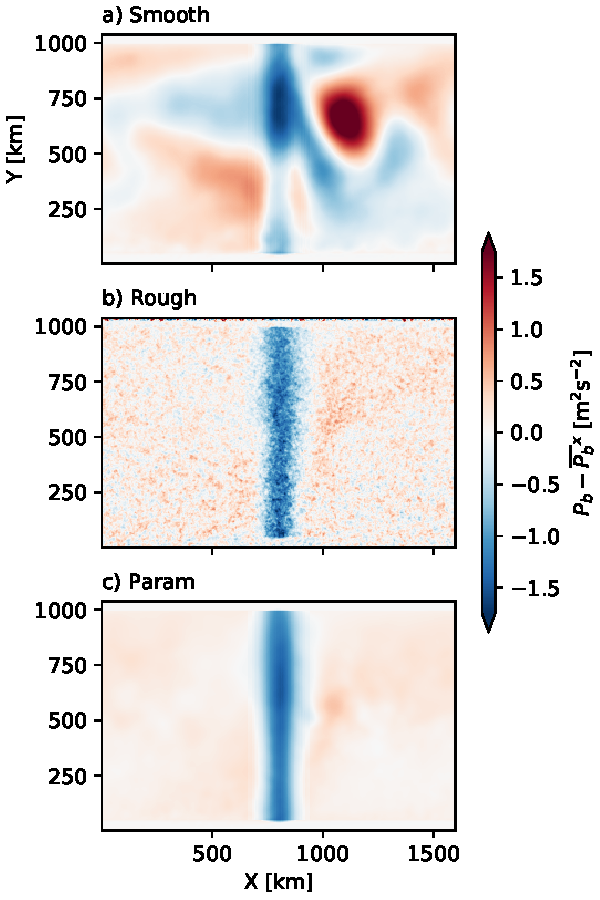
\includegraphics[width=\onewidth]{BottomPressure.pdf}
    \caption{Bottom pressure averaged over last two years of the simulation with the zonal means removed.  
      \tempS{\footnotesize ../figs/GetBottomDrag ;
        ../figs/BottomPressure.pdf}
      \label{fig:BottomPressure} }
  \end{center}
\end{figure}

\subsection{Integrated response and parameterization} 

The overall effect of the rough topography and the parameterization is to lead to smaller eddy kinetic energies by approximately 50\% (\fref{fig:TimeSeries305}a), and stronger downstream transport by up to a factor of four (\fref{fig:TimeSeries305}c).    The time series also make it clear that the simulations are in approximate mechanical steady state (\fref{fig:TimeSeries305}a), but that they have not reached thermal equilibrium (\fref{fig:TimeSeries305}b), which would take a few hundred years of simulation.  

\begin{figure}[htbp]
  \begin{center}
    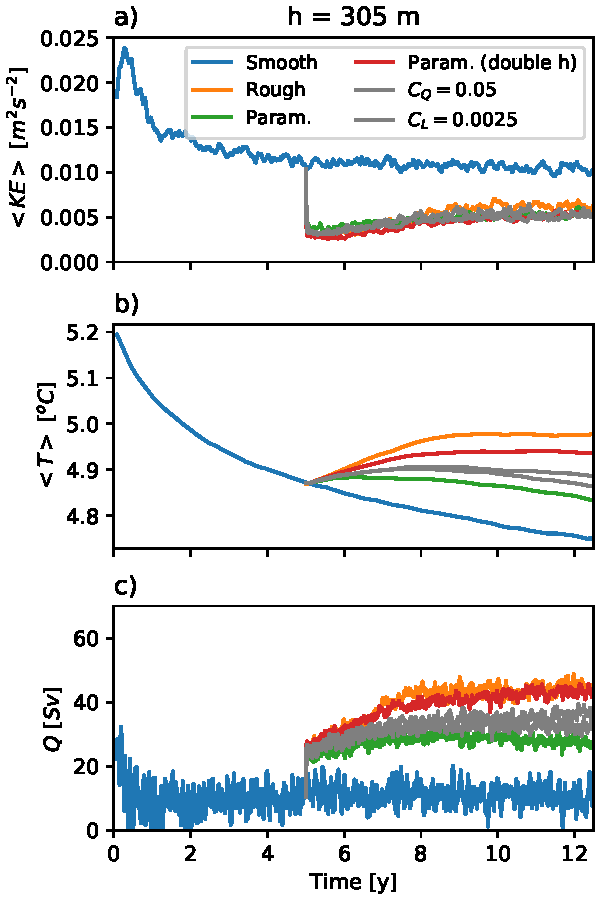
\includegraphics[width=\onewidth]{TimeSeries305}
    \caption{a) Model-mean kinetic energy in the simulations with various parameterizations of the drag.  b) Model-mean temperature c) Mean downstream transport.  {\sc Smooth} is with no roughness and weak quadratic drag, {\sc Rough} has stochastic bathymetry in the model, {\sc Param} is smooth bathymetry with a hybrid linear/quadratic parameterization given in \fref{eq:FormDragParam}, and the red curve is with the same parameterization but $h$ doubled.  $C_Q$ is with a heightened quadratic drag only, and $C_L$ is with a heightened linear drag only.  
      \tempS{\footnotesize ../figs///Notes5k ;
        ../figs//TimeSeries305.pdf}
      \label{fig:TimeSeries305} }
  \end{center}
\end{figure}

Parameterizing the drag due to the rough bathymetry was attempted a few different ways.  First, we tried a run with just a quadratic drag co-efficient of $C_Q=0.05$ and a separate run with just a linear drag co-efficient of $C_L=0.0025$.  These are quite high drag coefficients, and lead to a strong increase of the down-channel transport (\fref{fig:TimeSeries305}c), to 35 and 30 Sv respectively.  Our first attempt to parameterize the rough drag was n \fref{eq:FormDragParam} with $h=305\ \mathrm{m}$ as the amplitude of the bathymetry in the {\sc rough} simulations.  This direct use of the parameterization proposed above meant using $C_l = 7.3\times 10^{-4}$ and $C_q = 1.5\times 10^{-2}$ ({\sc param}) but leads to a downstream transport that is too weak (\fref{fig:TimeSeries305}c, green curve).  An ad-hoc doubling the ``effective'' value of $h$ in the parameterization to $610\ \mathrm{m}$ leads to a much closer parameterization of the downstream transport ({\sc Double}, \fref{fig:TimeSeries305}c, red curve).  

\begin{figure}[htbp]
  \begin{center} 
    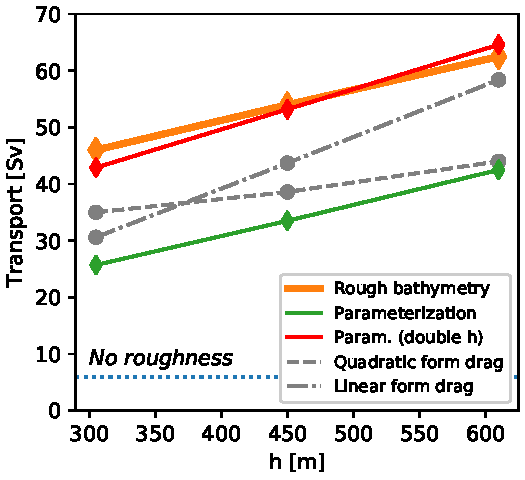
\includegraphics[width=2.5in]{VaryH}
    \caption{Effects on the downstream transport of different roughness parameterizations.  "Rough" is the 5-km simulations with resolved topography included.  "Parameterization" is the parameterization suggested in this paper. "Param. (double h)" (red) is the same parameterization, but with the topographic height doubled in the parameterization (i.e. peak-to-trough height).  Simulations with a quadratic (in velocity) form drag (grey dashed) and linear (in velocity) form drag only, roughly scaled to match the {\sc rough} simulations.  
      \tempS{\footnotesize ../figs///Notes5k ;
        ../figs//VaryH.pdf}
      \label{fig:VaryH} }
  \end{center}
\end{figure}

In these simulations, it is easiest to change the topographic amplitude, so we have done so over a range of topographic heights that are relatively large, 305 m (the cases shown above), 450 m, and 610 m. We ran the model with explicit rough bathymetry, and with parameterized drags.  For the linear-only drag law we increased the co-efficient by the square of the topographic height, and for the quadratic-only, we increased it linearly with the topographic height.  For the combined drag as proposed in this paper, we ran with both $h$ and $2h$.  

As the stochastic topographic amplitude $h$ is increased in the model simulations with explicit roughness, the downstream transport increases from 45 Sv to 62 Sv (\fref{fig:VaryH}, orange) due to the extra suppression of eddies.  The quadratic form drag is assumed to scale with $h$, and hence does not see as much an increase is downstream transport as $h$ is increased (\fref{fig:VaryH}, gray, dashed).  The linear form drag scales as $h^2$, and has a larger fractional increase in the downstream transport than is observed (\fref{fig:VaryH}, gray, dash-dot).  The parameterization (\fref{fig:VaryH}, green curve), and the version with {\sc Double} the topographic amplitude ((\fref{fig:VaryH}, red curve)  have  dependence on $h$ that is very similar to the explicit bathymetry simulation, and the {\sc Double} drag law with $2h$ also has the correct amplitudes.  Of course both the linear or quadratic drags could have been tuned to better match the rough simulations for any particular value of $h$, but the point is that the the dependence on other values of $h$ would still be incorrect, and that the hybrid scheme is an improvement over both.     

\clearpage
\section{Discussion}

Using the hybrid drag parameterization, \fref{eq:FormDragParam}, improves the simulation of bottom roughness as quantified by the downstream transport in the idealized wind-driven channel compared to runs with a linear or quadratic drag only.  There are a few straight-forward caveats to this finding that should be noted.  First, the body-forced runs (no wind forcing) found that the parameterization  should use the amplitude of the topographic spectrum, $h$ in \fref{eq:topo2d}. For the wind-forced runs, however, the drag from this formulation was too low and we empirically doubled the topographic height to $2h$.  The reason for this difference will bear future scrutiny, but one possibility is that the stratification evolves differently in each type of simulation.  In the wind-forced runs, any given parcel of topography sees low-frequency currents from different directions, and a continual input of dense water from the overturning circulation in the model.  The body-forced runs, on the other hand, have flow always from one direction, meaning large-scale regions of blocked unstratified flow can develop over the duration of the simulations.  This reduces the effective height of the topography \citep[i.e.][]{aguilarsutherland06}, and hence a reduced topographic height is accurate.  This stagnant region may not have the ability to form in the eddying model, so the peak-to-peak amplitude of the topography is a more appropriate scale.

A related issue is that when we applied the drag law to the eddying simulations we did not include the computational complexity of computing the stratification, and hence $N$ in the model, and instead used a constant for the parameterization.  This was just for convenience, and to see if the drag law was useful.  However, given that the linear drag depends on $N$, this really should be done online and be allowed to vary across the domain.   Similarly, we would expect substantial mixing from the parameterized drag, but we have not included this extra mixing in the simulations used here, and how this would feed back with the overturning circulation in the eddying simulations is an important question \citep{broadbridgeetal16}. However, as noted, we did not run the models to thermal equilibrium, so testing this would require significant more numerical expense.  

An important caveat is that all the topography used here is stochastic, isotropic, and homogenous across the domain.   These assumptions break down at the larger scales we are interested in here, perhaps much more so than the smaller-scale ``abyssal hills''  that radiate lee waves.  In particular, the effect of organized large-scale bathymetry rather than stochastic bathymetry should be investigated.  Anisotropy may particularly matter if the different topographic wavelengths are organized in such a way as to be random in one direction, and in-phase for others.  

Finally, the eddying simulations were somewhat cheaply run, and there is good evidence that changing the horizontal and vertical resolution can affect the near-bottom drag significantly in the presence of rough bathymetry \citep{klymak18}.  Our coarse ($\sim$40-m) vertical resolution also hampered our ability to look at smaller  topographic amplitudes. 

The overall importance of parameterizing the drag with an $Nh/u_0$ dependent hybrid between a linear drag and a quadratic one can be investigated by considering the bathymetry roughness parameterization as supplied by \citep{goffarbic10} and the global ocean data base of near-bottom ocean stratification (\fref{fig:GlobalMap}).  It is hard to compare the drag co-efficients because they have very different magnitudes, though the linear drag co-efficient can be seen to be large at many locations in the ocean.  If we choose a moderate eddying velocity of $U=0.08\ \mathrm{m\,s^{-1}}$, then we can directly compare the drags produced in such a map.  Overall, the quadratic drag dominates in most locations, but the regions where the quadratic drag is highest tend to be regions where the fraction of the total drag from the linear drag becomes more than 50\% (\fref{fig:GlobalMap}f), indicating that including the linear drag for high $Nh/u_0$ flows is valuable.  

%  TODO: Discuss othe papers with more resolution (i.e. Srinivassan).


\begin{figure*}[htbp]
  \begin{center}
    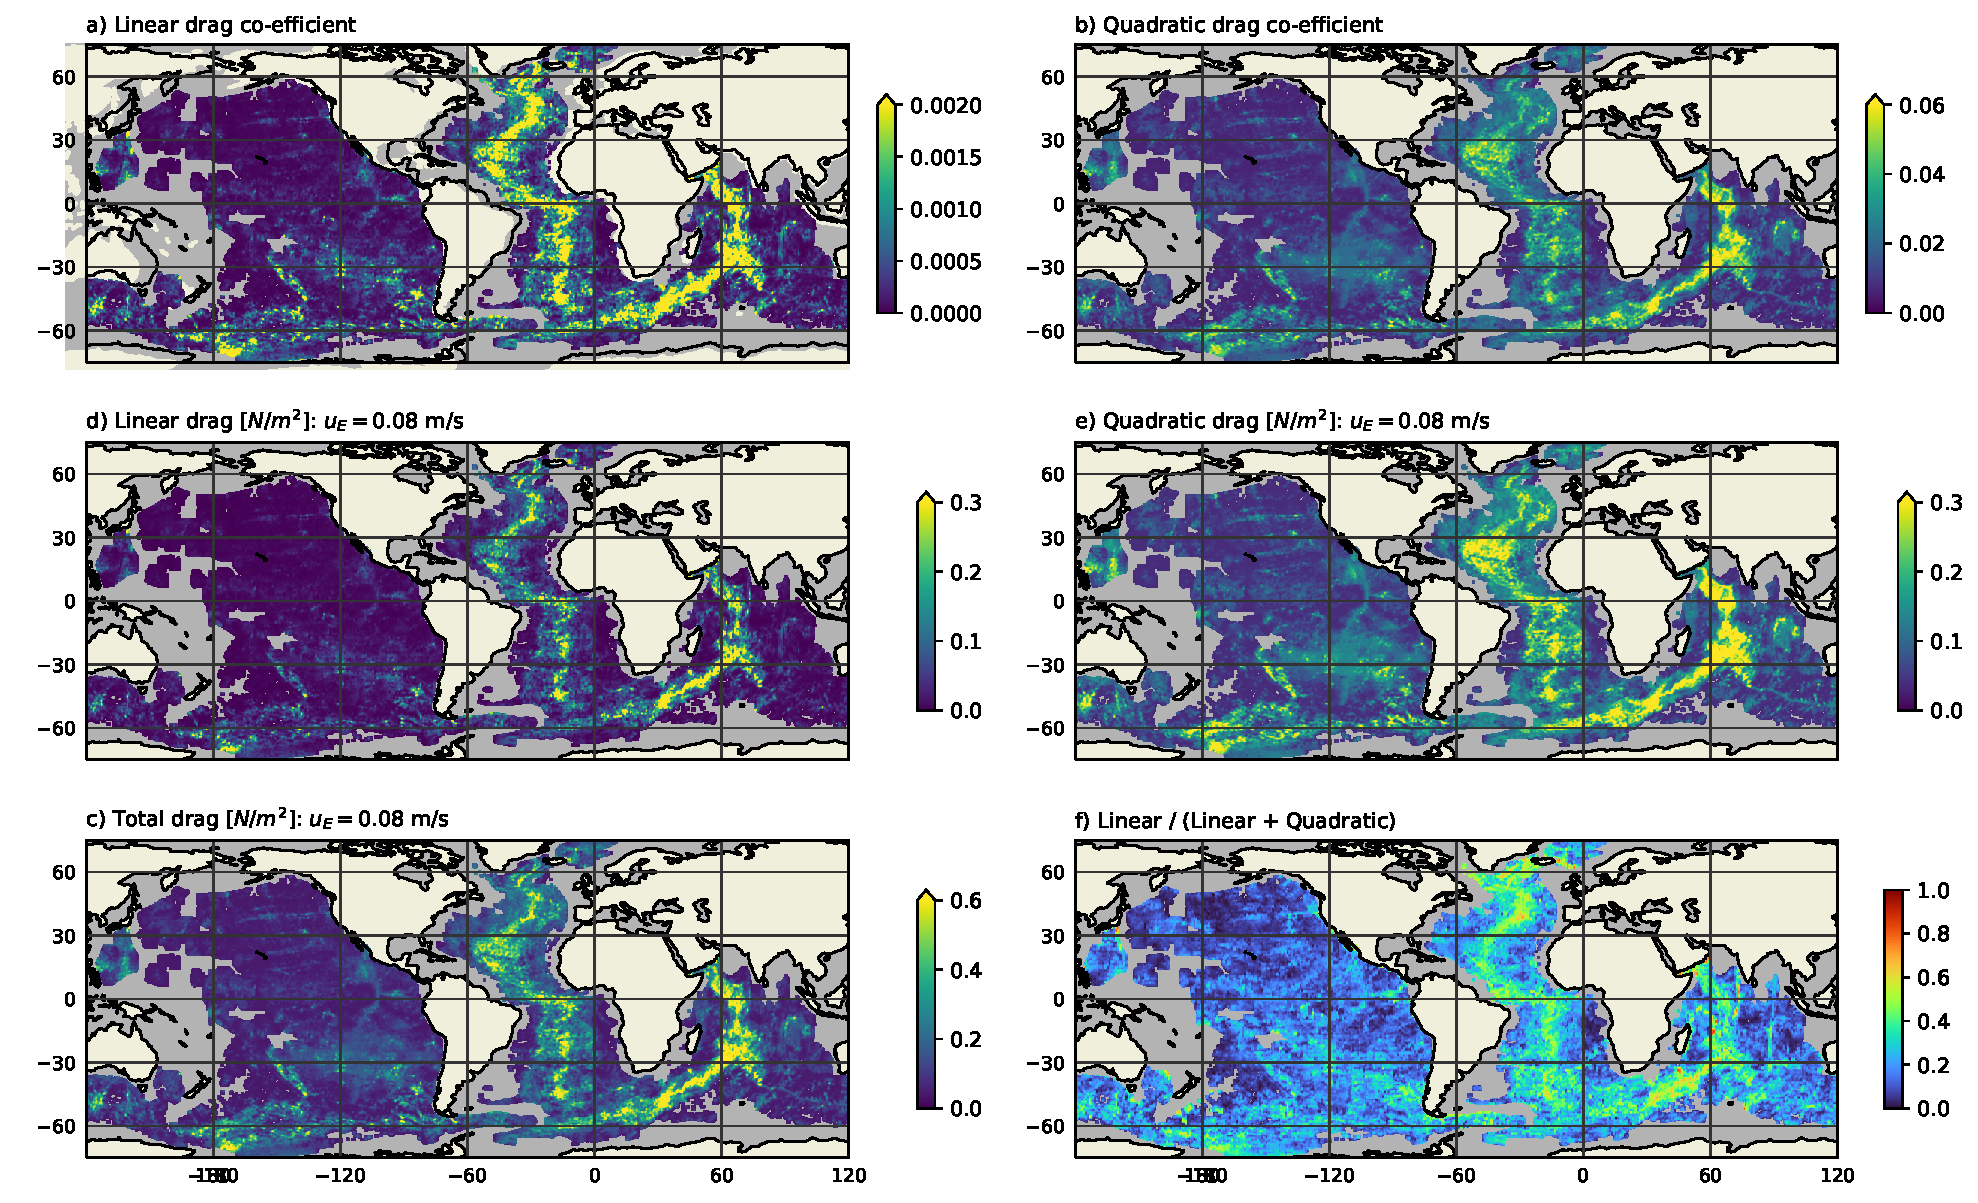
\includegraphics[width=6.75in]{/Users/jklymak/Dropbox/Goff_bathy/GoffResults.pdf}
    \caption{Drag co-efficients proposed in this paper
      \tempS{\footnotesize /Users/jklymak/ForcedChannel5k/Notes5k ;     
        /Users/jklymak/ForcedChannel5k/figs/TimeSeries_smoothvroughlindrag2kmZoom}
      \label{fig:GlobalMap} }
  \end{center}
\end{figure*}

The scheme presented here benefits from substantial simplicity while retaining a $Nh/u_0$ dependence on the cross-over between the linear drag regime and the quadratic.  To our knowledge, simulations have either used the linear or quadratic drag laws exclusively, and not used this hybrid approach.  The lee-wave parameterizations \citep[i.e.][]{nikurashinferrari14} work out to be linear drag laws, and the parameterizations that in addition account for non-propagating effects \citep[][]{trossmanetal13, trossmanetal2016} also are implemented as a linear drag with a geometric amplification.  Conversely, non-propagating drag in the atmosphere is typically parameterized as a quadratic drag \citep{LottMiller97, ScinoccaMcFarlane00}.  Certainly, there are values of $Nh/U$ that are large enough in the atmosphere to mean that the linear part of the drag law suggested here is important.  


%\begin{appendix}
%%%%%%%%%%%%%%%%%%%%%%%%%%%%%%%%%%%%%%%%%%%%%%%%%%%%%%%%%%%%%%%%%%%%%
% ACKNOWLEDGMENTS
%%%%%%%%%%%%%%%%%%%%%%%%%%%%%%%%%%%%%%%%%%%%%%%%%%%%%%%%%%%%%%%%%%%%%
\acknowledgments

This work was funded under the Office of Naval Research Flow Encountering Abrupt Topography Defence Research Initiative (grant N00014-15-1-2585), and NSERC Discovery Grant 327920-2006.  Thanks to Odessa Murray who manages the High Performance Computing accounts for ONR.  


%\subsection{First appendix secondary heading}
%
%\subsection{Second appendix secondary heading}
%
%\subsubsection{First appendix tertiary heading}
%
%\subsubsection{Second appendix tertiary heading}
%
%\paragraph{First appendix quaternary heading}
%
%\paragraph{Second appendix quaternary heading}
%
%\end{appendix}

% Create a bibliography directory and place your .bib file there.
% -REMOVE ALL DIRECTORY PATHS TO REFERENCE FILES BEFORE SUBMITTING TO THE AMS FOR PEER REVIEW

\bibliographystyle{ametsoc2014}
\bibliography{main}

%%%%%%%%%%%%%%%%%%%%%%%%%%%%%%%%%%%%%%%%%%%%%%%%%%%%%%%%%%%%%%%%%%%%%
% FIGURES-REMOVE ALL DIRECTORY PATHS TO FIGURE FILES BEFORE SUBMITTING TO THE AMS FOR PEER REVIEW
%%%%%%%%%%%%%%%%%%%%%%%%%%%%%%%%%%%%%%%%%%%%%%%%%%%%%%%%%%%%%%%%%%%%%

%
\end{document}
